\documentclass[../notes.tex]{subfiles}

\pagestyle{main}
\renewcommand{\chaptermark}[1]{\markboth{\chaptername\ \thechapter\ (#1)}{}}
\setcounter{chapter}{5}

\begin{document}




\chapter{Thermodynamics}
\section{Selectivity}
\begin{itemize}
    \item \marginnote{10/8:}Lecture 9 recap.
    \begin{itemize}
        \item Last lecture wrapped up reactive intermediates, focusing specifically on carbenes.
        \item Triplet carbenes (Figure \ref{fig:carbeneSTa}).
        \begin{itemize}
            \item More linear.
            \item Smaller HOMO-LUMO gap implies 2 SOMOs.
            \item React as diradicals.
            \item \ce{R} can be any $\pi$-acceptor, such as alkyl, vinyl, aryl, carbonyl, \ce{SO2R}, \ce{NO2}, \ce{B}, etc. groups.
        \end{itemize}
        \item Singlet carbenes (Figure \ref{fig:carbeneSTb}).
        \begin{itemize}
            \item More bent.
            \item Larger HOMO-LUMO gap.
            \item React as cations and anions.
            \item \ce{R} can be any $\pi$-donor or $\sigma$-EWG, such as halogens, \ce{NR2}, or \ce{OR} groups.
        \end{itemize}
        \item Both types of carbenes\dots
        \begin{itemize}
            \item Can be nucleophilic or electrophilic;
            \item React by adding into $\pi$-systems or inserting into bonds.
            \begin{itemize}
                \item The mechanisms through which S/T carbenes engage in this reactivity vary slightly.
            \end{itemize}
        \end{itemize}
    \end{itemize}
    \item Today: Selectivity.
    \item Lecture outline.
    \begin{itemize}
        \item Thermodynamic selectivity.
        \item Kinetic selectivity.
        \item Curtin-Hammett kinetics.
        \item Kinetic quench.
        \item Principle of microscopic reversibility.
        \item Reactivity-selectivity principle.
        \item Practical aspects of selectivity (deferred to next time).
    \end{itemize}
    \item When two products form from a single common intermediate (or starting material), selectivity between these products can arise from \textbf{thermodynamic} or \textbf{kinetic} factors.
    \pagebreak
    \item \textbf{Thermodynamic} (selectivity): Selecting for a certain product based on the position of an equilibrium, i.e., the stability of the products.
    \begin{figure}[h!]
        \centering
        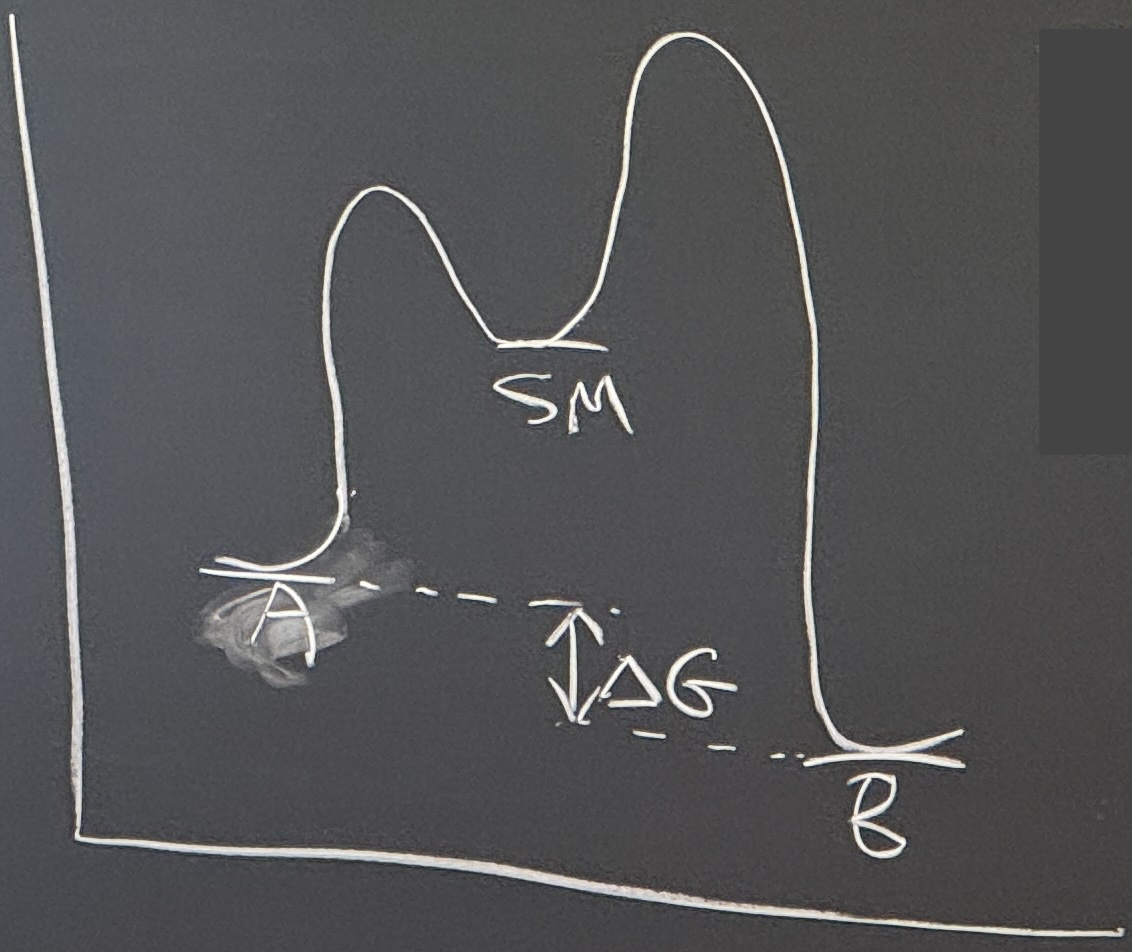
\includegraphics[width=0.2\linewidth]{EstabTherm.JPG}
        \caption{Energy variables relevant to thermodynamic selectivity.}
        \label{fig:EstabTherm}
    \end{figure}
    \begin{itemize}
        \item Key words: Thermodynamic = product = equilibrium.
        \item Relevant reaction coordinate.
        \begin{equation*}
            \ce{A <=>[$K_{\ce{A}}$] SM <=>[$K_{\ce{B}}$] B}
        \end{equation*}
        \begin{itemize}
            \item \ce{A} and \ce{B} form from a single common starting material (SM).
            \item The relevant equilibrium constants are $K_{\ce{A}}$ and $K_{\ce{B}}$.
        \end{itemize}
        \item $K_{\ce{A}}$ and $K_{\ce{B}}$ allow us to define the \textbf{selectivity} of this reaction as follows.
        \begin{equation*}
            \text{selectivity} = \frac{\cnc{A}}{\cnc{B}}
            = \frac{K_{\ce{A}}}{K_{\ce{B}}}
            =: \Keq
        \end{equation*}
        \item Energy diagram of a thermodynamically controlled reaction (Figure \ref{fig:EstabTherm}).
        \begin{itemize}
            \item In order for a reaction to be under thermodynamic control, all steps must be reversible, i.e., all intermediates must interconvert.
            \item $\Delta G$ is the difference in energy between the products.
            \item Recall from Gen Chem that $\Delta G=-RT\ln(\Keq)$ and hence $\Keq=\e[-\Delta G/RT]$.
        \end{itemize}
        \item Thermodynamic selectivity is very useful if all products are at very different energy levels.
        \item Example: Olefin isomerization can occur with great selectivity because one product can be much more stable than another.
    \end{itemize}
    \item \textbf{Selectivity} (of a reaction): The preference for one product (\ce{A}) over another (\ce{B}), where both \ce{A} and \ce{B} originate from a single common intermediate or starting material. \emph{Given by}
    \begin{equation*}
        \text{selectivity} := \frac{\cnc{A}}{\cnc{B}}
    \end{equation*}
    \item \textbf{Kinetic} (selectivity): Selecting for a certain product based on the differences in energies of competing transition states, i.e., by reaction rates.
    \begin{figure}[H]
        \centering
        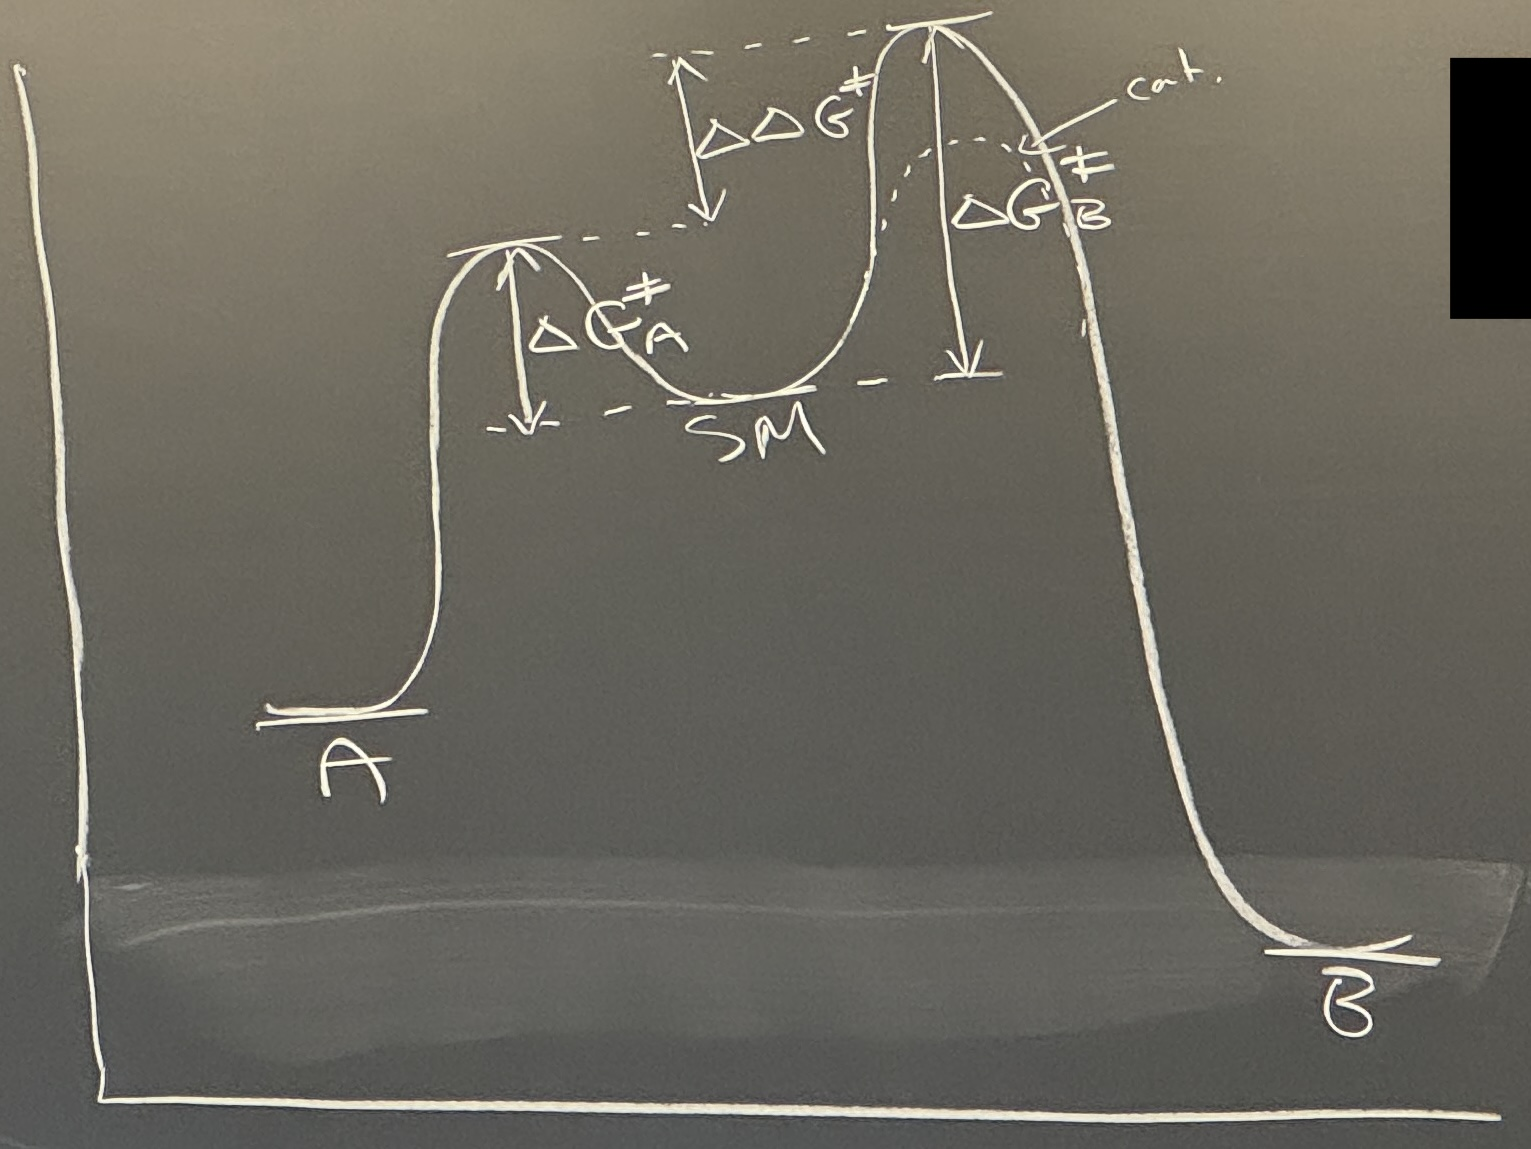
\includegraphics[width=0.35\linewidth]{EstabKin.JPG}
        \caption{Energy variables relevant to kinetic selectivity.}
        \label{fig:EstabKin}
    \end{figure}
    \begin{itemize}
        \item Key words: Kinetic = transition state = rate.
        \item Relevant reaction coordinate.
        \begin{equation*}
            \ce{A <-[$k_{\ce{A}}$] SM ->[$k_{\ce{B}}$] B}
        \end{equation*}
        \begin{itemize}
            \item As before, \ce{A} and \ce{B} form from a single common SM.
            \item The relevant rate constants are $k_{\ce{A}}$ and $k_{\ce{B}}$.
        \end{itemize}
        \item $k_{\ce{A}}$ and $k_{\ce{B}}$ allow us to define the selectivity of this reaction as follows.
        \begin{equation*}
            \text{selectivity} = \frac{\cnc{A}}{\cnc{B}}
            = \frac{k_{\ce{A}}}{k_{\ce{B}}}
        \end{equation*}
        \item Energy diagram of a kinetically controlled reaction (Figure \ref{fig:EstabKin}).
        \begin{itemize}
            \item $\Delta G_{\ce{A}}^\ddagger$ and $\Delta G_{\ce{B}}^\ddagger$ are the activation energies required to form the transition states from the SM to \ce{A} and \ce{B}, respectively.
            \item $\Delta\Delta G^\ddagger$ is then the difference between these transition states' activation energies.
            \item Recall from Gen Chem that $\Delta\Delta G^\ddagger=-RT\ln(k_{\ce{A}}/k_{\ce{B}})$.\footnote{This can be derived by dividing the Arrhenius equation for one reaction by the Arrhenius equation for the other reaction and rearranging.}
            \item Often, $k_{\ce{A}}/k_{\ce{B}}$ is equal to the relative rate $\krel$ of the two reactions (\ce{SM -> A} and \ce{SM -> B}).
            \begin{itemize}
                \item If \ce{A} and \ce{B} are enantiomers or diastereomers, $\krel$ often equals \textbf{er} or \textbf{dr}, respectively.
                \item Another consequence of the introduction of $\krel$ is that $\krel=\e[-\Delta\Delta G^\ddagger/RT]$.
            \end{itemize}
            \item Note that \emph{catalyzing} a pathway is a kinetic effect, corresponding to a lower activation barrier.
        \end{itemize}
        \item In contrast to thermodynamic equilibrium, the products formed here are formed irreversibly and do not interconvert.
        \item Kinetic control is more common than thermodynamic control.
        \begin{itemize}
            \item Reactions under thermodynamic control have largely been developed and optimized over the last 100 years, so kinetic control gives us a better handle in modern methods development.
            \item Everything about a catalytic cycle is based on kinetics! You're not changing the thermodynamics of \ce{CO2} upcycling; you're making it more energetically feasible.
        \end{itemize}
    \end{itemize}
    \item \textbf{Enantiomeric ratio}: The ratio of the (\emph{S})-enantiomer to the (\emph{R})-enantiomer. \emph{Denoted by} \textbf{er}.
    \begin{itemize}
        \item This is more mathematically useful than the enantiomeric excess (ee), so there's currently something of a push to phase out ee in favor of er.
        \item ee is still used primarily for historical reasons.
    \end{itemize}
    \item \textbf{Diasteriomeric ratio}: The ratio of one diastereomer to the other. \emph{Denoted by} \textbf{dr}.
    \item We now discuss a special type of kinetic control called \textbf{Curtin-Hammett kinetics}.
    \item \textbf{Curtin-Hammett} (kinetics): A kinetic regime characterized by two starting materials or intermediates that rapidly interconvert, causing the ratio of products (i.e., the selectivity) to depend only on the transition state energies. \emph{Also known as} \textbf{C/H}.
    \begin{figure}[H]
        \centering
        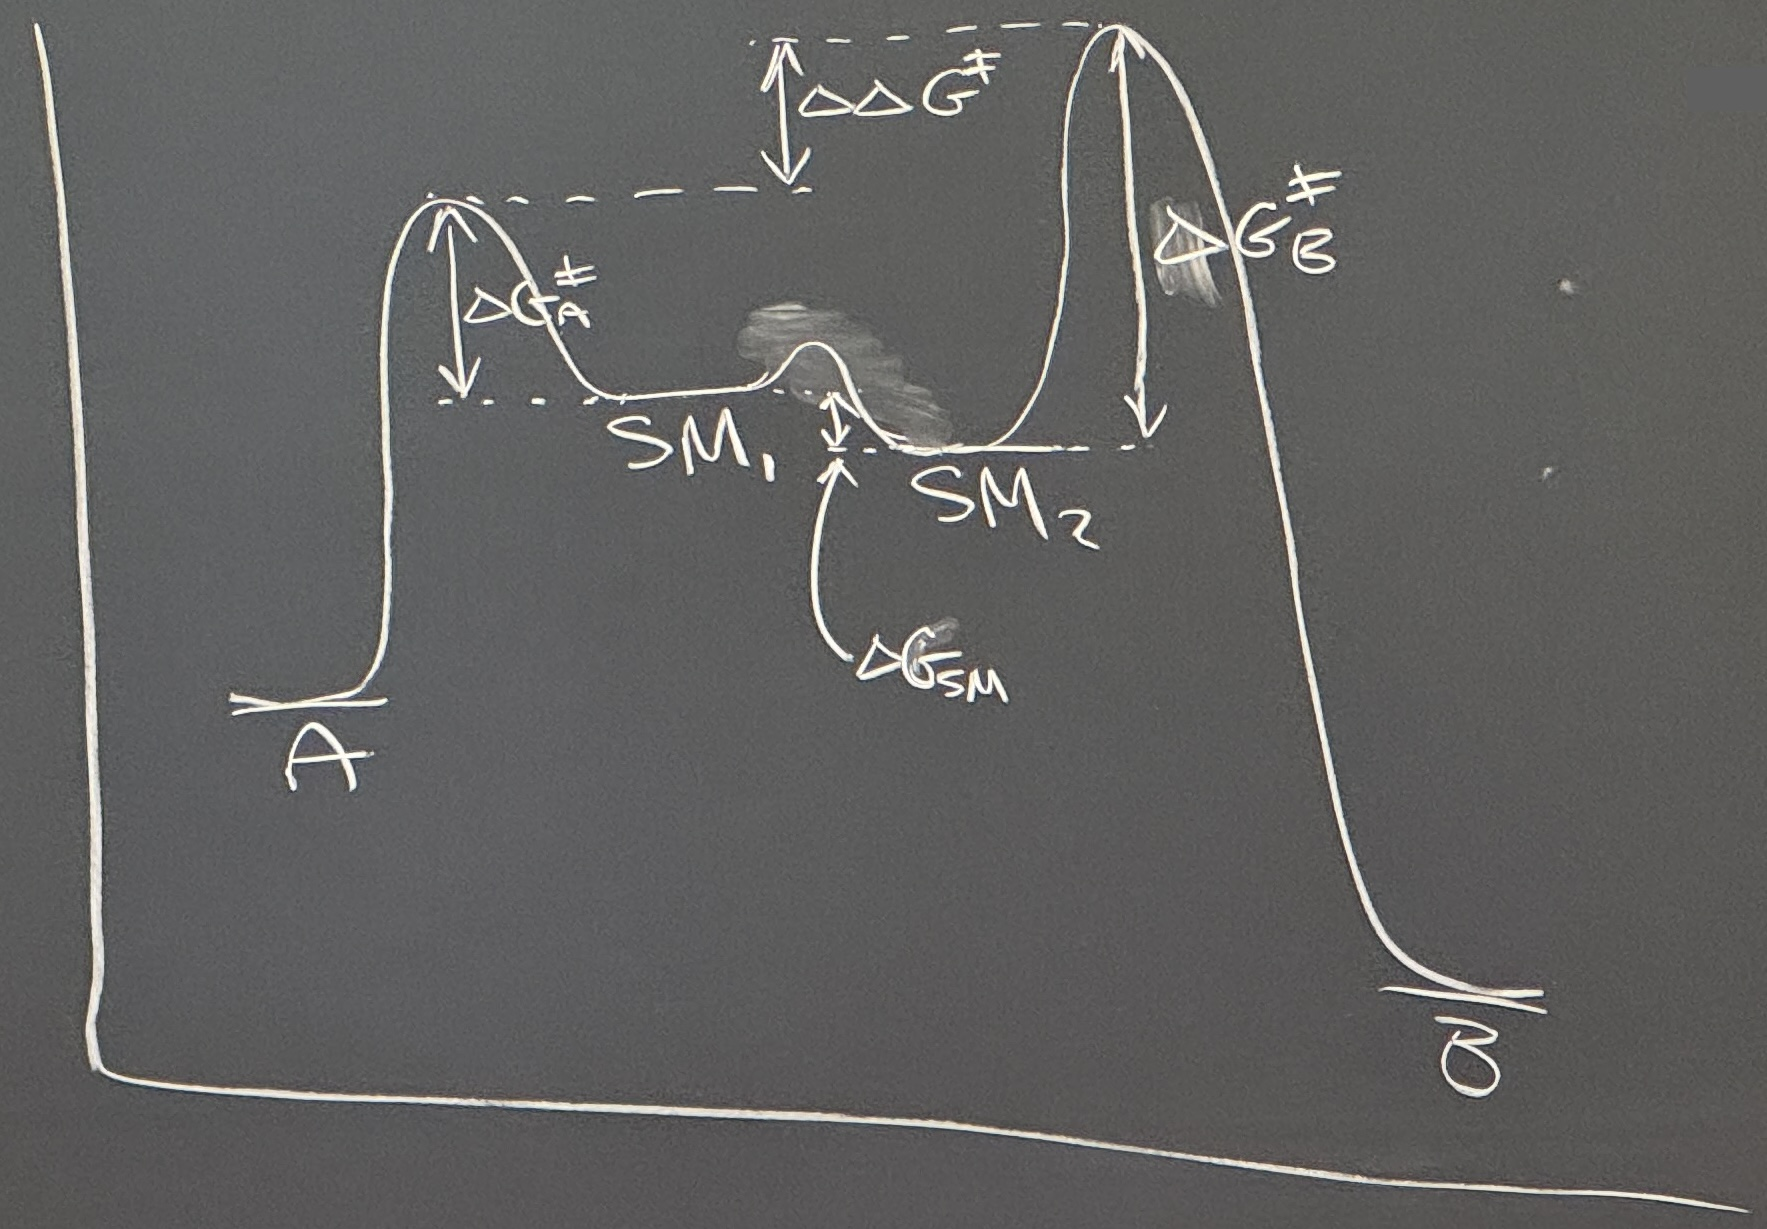
\includegraphics[width=0.35\linewidth]{EvarCH.JPG}
        \caption{Energy variables relevant to Curtin-Hammett kinetics.}
        \label{fig:EvarCH}
    \end{figure}
    \begin{itemize}
        \item In particular, the selectivity does \emph{not} depend on the energies of the starting materials.
        \item Relevant reaction coordinate.
        \begin{equation*}
            \ce{A <-[$k_{\ce{A}}$] SM1 <=>[$K_\text{SM}$][$k_\text{SM}$] SM2 ->[$k_{\ce{B}}$] B}
        \end{equation*}
        \begin{itemize}
            \item $k_\text{SM}$ must be big. Typically, it is approximately ten times faster than $k_{\ce{A}}$ or $k_{\ce{B}}$.
        \end{itemize}
        \item Working out the math, we get
        \begin{equation*}
            \text{selectivity} = \frac{\cnc{A}}{\cnc{B}}
            = \e[-\Delta\Delta G^\ddagger/RT]
        \end{equation*}
        \begin{itemize}
            \item Indeed, we see that in this regime, the selectivity \emph{mathematically} depends only on the relative energies of the transition states.
        \end{itemize}
        \item Energy diagram of a reaction under Curtin-Hammett kinetics (Figure \ref{fig:EvarCH}).
        \begin{itemize}
            \item Note that there is only a small energy barrier between \ce{SM1} and \ce{SM2} because we need fast interconversion.
        \end{itemize}
        \item Observe that the products are formed irreversibly and do not interconvert.
        \begin{itemize}
            \item Indeed, the SMs interconvert freely as long as they stay SMs, but once they go over their barrier to \ce{A} or \ce{B}, they do not continue to interconvert.
        \end{itemize}
    \end{itemize}
    \item Scenarios that manifest Curtin-Hammett kinetics.
    \begin{figure}[h!]
        \centering
        \begin{subfigure}[b]{0.33\linewidth}
            \centering
            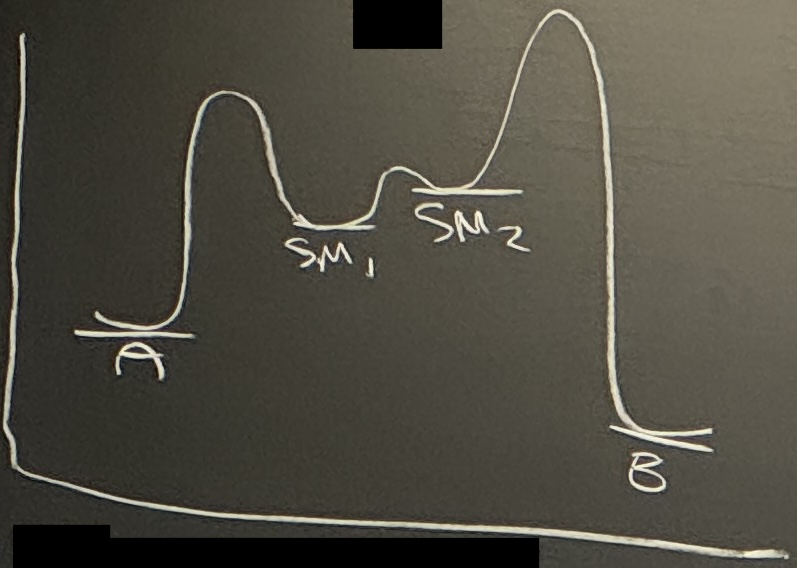
\includegraphics[width=0.79\linewidth]{CHscenarioa.JPG}
            \caption{More stable reacts more quickly.}
            \label{fig:CHscenarioa}
        \end{subfigure}
        \begin{subfigure}[b]{0.32\linewidth}
            \centering
            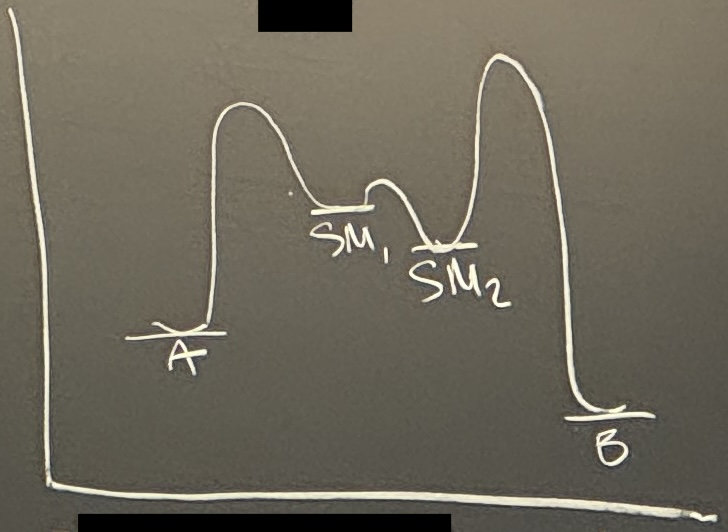
\includegraphics[width=0.8\linewidth]{CHscenariob.JPG}
            \caption{Less stable reacts more quickly.}
            \label{fig:CHscenariob}
        \end{subfigure}
        \begin{subfigure}[b]{0.33\linewidth}
            \centering
            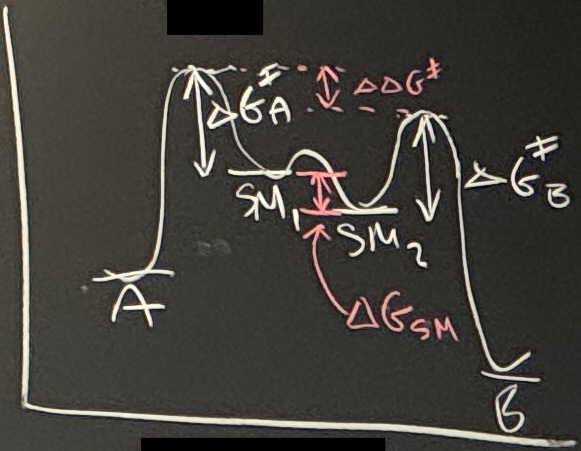
\includegraphics[width=0.74\linewidth]{CHscenarioc.JPG}
            \caption{Both react same.}
            \label{fig:CHscenarioc}
        \end{subfigure}
        \caption{Curtin-Hammett scenarios.}
        \label{fig:CHscenario}
    \end{figure}
    \begin{enumerate}
        \item The more stable starting material reacts more quickly (Figure \ref{fig:CHscenarioa}).
        \begin{itemize}
            \item Let \ce{SM1} be lower energy than \ce{SM2}, and let the \ce{SM1 -> A} transition state have a lower activation energy than the \ce{SM2 -> B} transition state.
            \item It follows that \ce{SM1} is thermodynamically favored. This means that we'll see more of it in solution: $\cnc{SM1}>\cnc{SM2}$.
            \item The lower activation energy to form \ce{A} (i.e., $\Delta G_{\ce{A}}^\ddagger<\Delta G_{\ce{B}}^\ddagger$) implies that \ce{A} is kinetically favored.
            \item The product ratio will not be equal to the starting material ratio.
            \begin{itemize}
                \item You might not even see \ce{SM2} among the starting materials; you might just think that \ce{SM1 -> A + B}.
            \end{itemize}
            \item Takeaway: It isn't always obvious when Curtin-Hammett kinetics are in effect.
        \end{itemize}
        \item The less stable starting material reacts more quickly (Figure \ref{fig:CHscenariob}).
        \begin{itemize}
            \item Let \ce{SM1} be higher energy than \ce{SM2}, and let the \ce{SM1 -> A} transition state have a lower activation energy than the \ce{SM2 -> B} transition state.
            \item It follows that \ce{SM2} is thermodynamically favored. This means that we'll see more of it in solution: $\cnc{SM2}>\cnc{SM1}$.
            \item The lower activation energy to form \ce{A} (i.e., $\Delta G_{\ce{A}}^\ddagger<\Delta G_{\ce{B}}^\ddagger$) implies that \ce{A} is kinetically favored.
            \item The less stable starting material is kinetically favored to react.
            \item Takeaway: All the reactivity goes through \ce{SM1}, even though we might not even see \ce{SM1}; you might just think that \ce{SM2 -> A + B}.
            \item This is classic Curtin-Hammett kinetics, wherein the product we observe is from the starting material we don't observe.
            \begin{itemize}
                \item Results like this can be confusing because the SM we put in the flask doesn't look like it'd give the product we see.
                \item This contrasts with Scenario 1, wherein the SM we see logically leads to our product \ce{A}, and all we miss is that there's a secret equilibrium that helps us get to \ce{B}.
            \end{itemize}
        \end{itemize}
        \item Both starting materials react equally quickly (Figure \ref{fig:CHscenarioc}).
        \begin{itemize}
            \item Let \ce{SM1} be higher energy than \ce{SM2}, and let the \ce{SM1 -> A} and \ce{SM2 -> B} transition states have identical activation energies (i.e., $\Delta G_{\ce{A}}^\ddagger=\Delta G_{\ce{B}}^\ddagger$).
            \item We call this \textbf{ground state control}.
            \begin{itemize}
                \item Thus, $\Delta G_{\ce{SM}}$ suddenly predicts our products; not because it actually does but because $\Delta\Delta G^\ddagger=\Delta G_{\ce{SM}}$.
                \item To reiterate: $\Delta\Delta G^\ddagger$ still controls selectivity; it just happens that it equals $\Delta G_{\ce{SM}}$.
            \end{itemize}
            \item Because $\Delta\Delta G^\ddagger=\Delta G_{\ce{SM}}$, we can work out mathematically that the selectivity happens to be the following (even though we still have C/H kinetics).
            \begin{equation*}
                \text{selectivity} = \frac{\cnc{A}}{\cnc{B}}
                = \frac{\cnc{SM1}}{\cnc{SM2}}
            \end{equation*}
            \item This regime often arises when \ce{A} and \ce{B} are really similar and hence have similar transition states (e.g., if \ce{A} and \ce{B} are enantiomers or diastereomers with far apart stereogenic centers).
        \end{itemize}
    \end{enumerate}
    \item It's our job as the responsible scientist to account for the full kinetic picture, even when it may not provide us much additional information!
    \begin{itemize}
        \item Indeed, the reactions that are the most interesting to develop are the ones that fall in this C/H regime because they have the most subtle reactivity.
    \end{itemize}
    \item Let's now look at some examples.
    \begin{itemize}
        \item Pay attention, because this is going to be a super useful skill for grad school and beyond!!
    \end{itemize}
    \item Example: Nitrogen rapidly epimerizes while a \emph{tert}-butyl group locks the chair in place.
    \begin{figure}[h!]
        \centering
        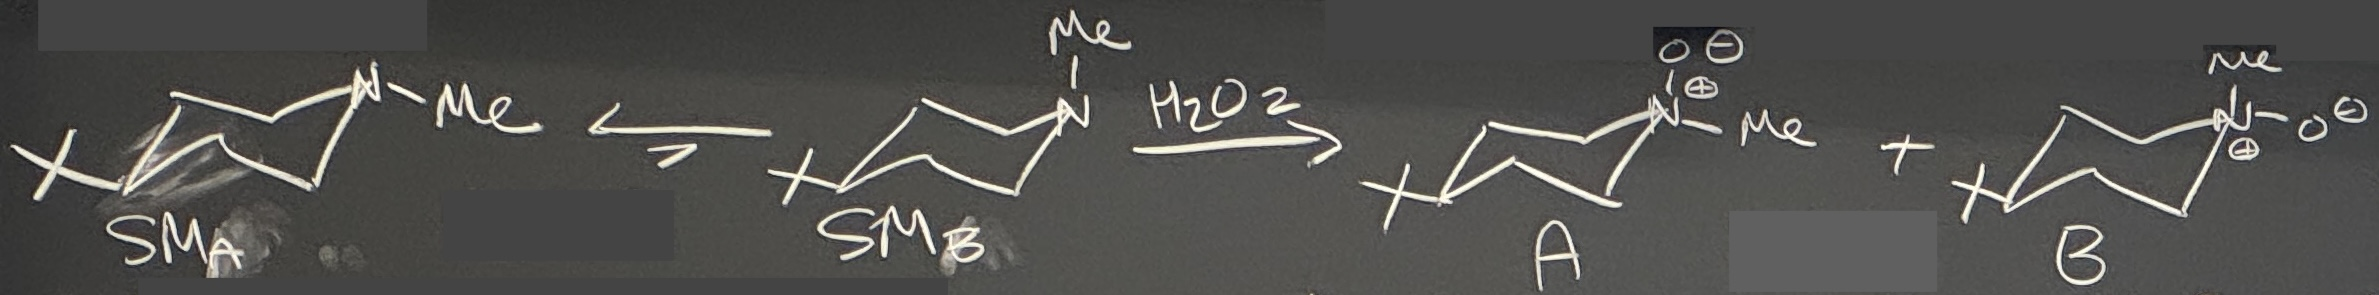
\includegraphics[width=0.6\linewidth]{CHepimers.JPG}
        \caption{Curtin-Hammett kinetics: Kinetically trapping epimers.}
        \label{fig:CHepimers}
    \end{figure}
    \begin{itemize}
        \item This epimerization (a \textbf{nitrogen inversion}) occurs fast relative to product formation.
        \item It puts \ce{SM_A} and \ce{SM_B} in a $98:2$ ratio.
        \item Either epimer can react with \ce{H2O2} to form the \emph{N}-oxo products in a $5:95$ ($\ce{A}:\ce{B}$) ratio.
        \item This is an example of Scenario 2 (Figure \ref{fig:CHscenariob}).
        \begin{itemize}
            \item Your first thought might be that the oxidation occurs with inversion of stereochemistry. This is a great first thought.
            \item But then you have to ask about alternate scenarios, and you should think about decoupled Curtin-Hammett steps wherein you're just kinetically trapping the epimers.
        \end{itemize}
    \end{itemize}
    \item Example: Axial and equatorial tosylates equilbriate before E\textsubscript{2} elimination to form a double bond.
    \begin{figure}[H]
        \centering
        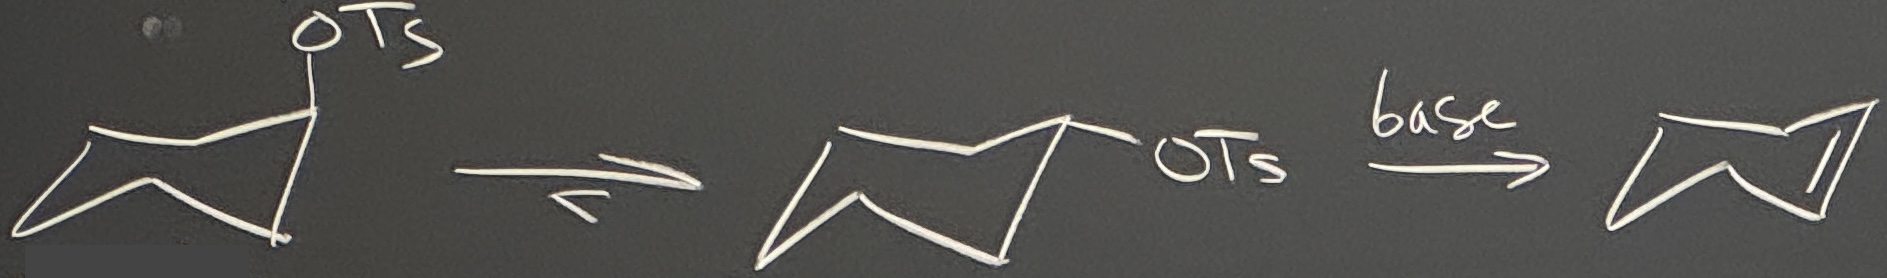
\includegraphics[width=0.4\linewidth]{CHelim.JPG}
        \caption{Curtin-Hammett kinetics: Elimination.}
        \label{fig:CHelim}
    \end{figure}
    \begin{itemize}
        \item Let \ce{SM_A} be the axial tosylate (on the left), and let \ce{SM_B} be the equatorial tosylate (on the right).
        \item Because of the large steric bulk of the tosylate group and hence its disfavored 1,3-diaxial interactions, \ce{SM_A} and \ce{SM_B} occur in a $1:14$ ratio.
        \item However, \ce{SM_A} has hydrogens antiperiplanar to it, so it reacts faster ($\krel=70$).
        \item So to recap: \ce{SM_B} is preferred, but the product comes from \ce{SM_A}. Therefore, this must be another example of Scenario 2 (Figure \ref{fig:CHscenariob}).
    \end{itemize}
    \item Example: \emph{trans} and \emph{cis} alkenes react via bromination to form a \emph{trans}- and \emph{cis}-dibromide.
    \begin{figure}[h!]
        \centering
        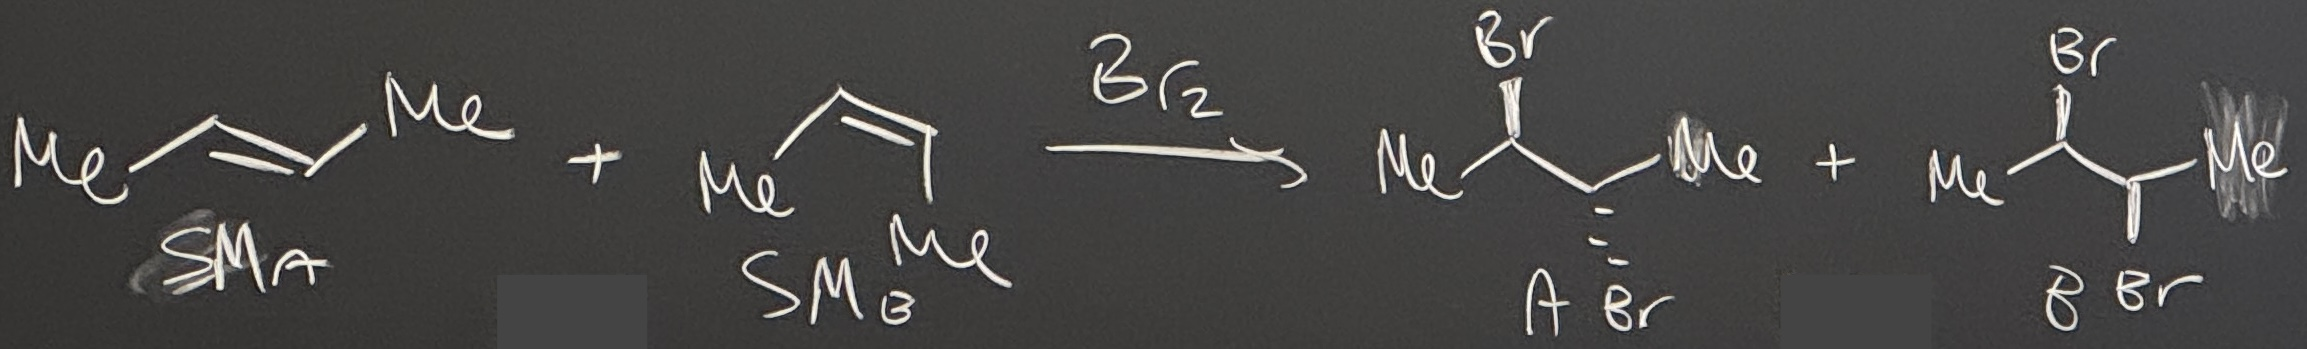
\includegraphics[width=0.5\linewidth]{CHgeometric.JPG}
        \caption{Curtin-Hammett kinetics: Bromination of geometric isomers.}
        \label{fig:CHgeometric}
    \end{figure}
    \begin{itemize}
        \item We have a $1:1$ mixture of SMs, and we form a $1:1$ mixture of products.
        \item Thus, based on the selectivity equation, it looks like this could be a candidate for Scenario 3. However, this is not C/H because the SMs do not interconvert! Rather, this is a case of a kinetic quench, which we'll cover next.
    \end{itemize}
    \item Learn C/H because we will see a lot of it on PSet 2.
    \item Kinetic quench (not C/H).
    \begin{figure}[h!]
        \centering
        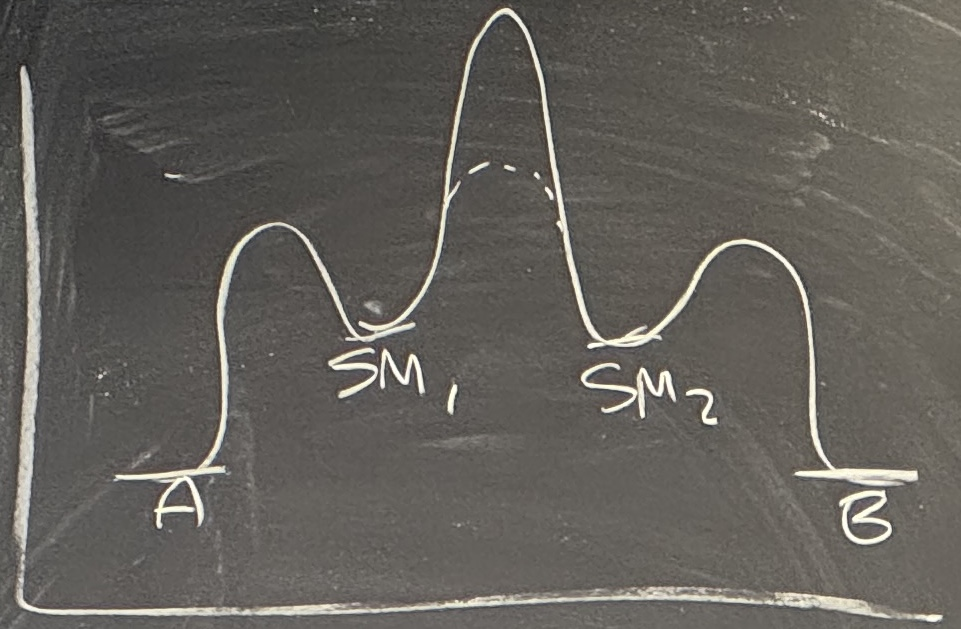
\includegraphics[width=0.25\linewidth]{EvarKQ.JPG}
        \caption{Energy variables relevant to a kinetic quench.}
        \label{fig:EvarKQ}
    \end{figure}
    \begin{itemize}
        \item Here, the \ce{SM1 <=> SM2} interconversion is slower than product formation.
        \item Thus, the ratio of starting materials equals the ratio of products, as follows.
        \begin{equation*}
            \text{product ratio} = \frac{\cnc{A}}{\cnc{B}}
            = \frac{\cnc{SM1}}{\cnc{SM2}}
        \end{equation*}
        \item This is basically a case of two isolated systems (\ce{SM1 -> A} and \ce{SM2 -> B}).\footnote{Could I come up with one-pot reactions where you have two different starting materials under kinetic quench form two different products and then those products react??}
        \pagebreak
        \item One tricky thing: When the rate of interconversion approximately equals the rate of product formation (Masha shows this regime with the dotted line in Figure \ref{fig:EvarKQ}).
        \begin{itemize}
            \item In this case, the product ratio is difficult to predict!
            \item That's real, messy science.
            \item When you encounter such a regime, either you change something to make it simpler, or you do a Wendlandt-style deep dive on the full mechanism where you uncover the secrets of the universe and then publish a bunch of \emph{Science} papers.
            \item "Alison's the master of these really hairy and difficult kinetic pictures and disentangling them and adding to our understanding of chemistry overall."
        \end{itemize}
    \end{itemize}
    \item Example of kinetic quench: Protonating two different epimers of an amine.
    \begin{figure}[h!]
        \centering
        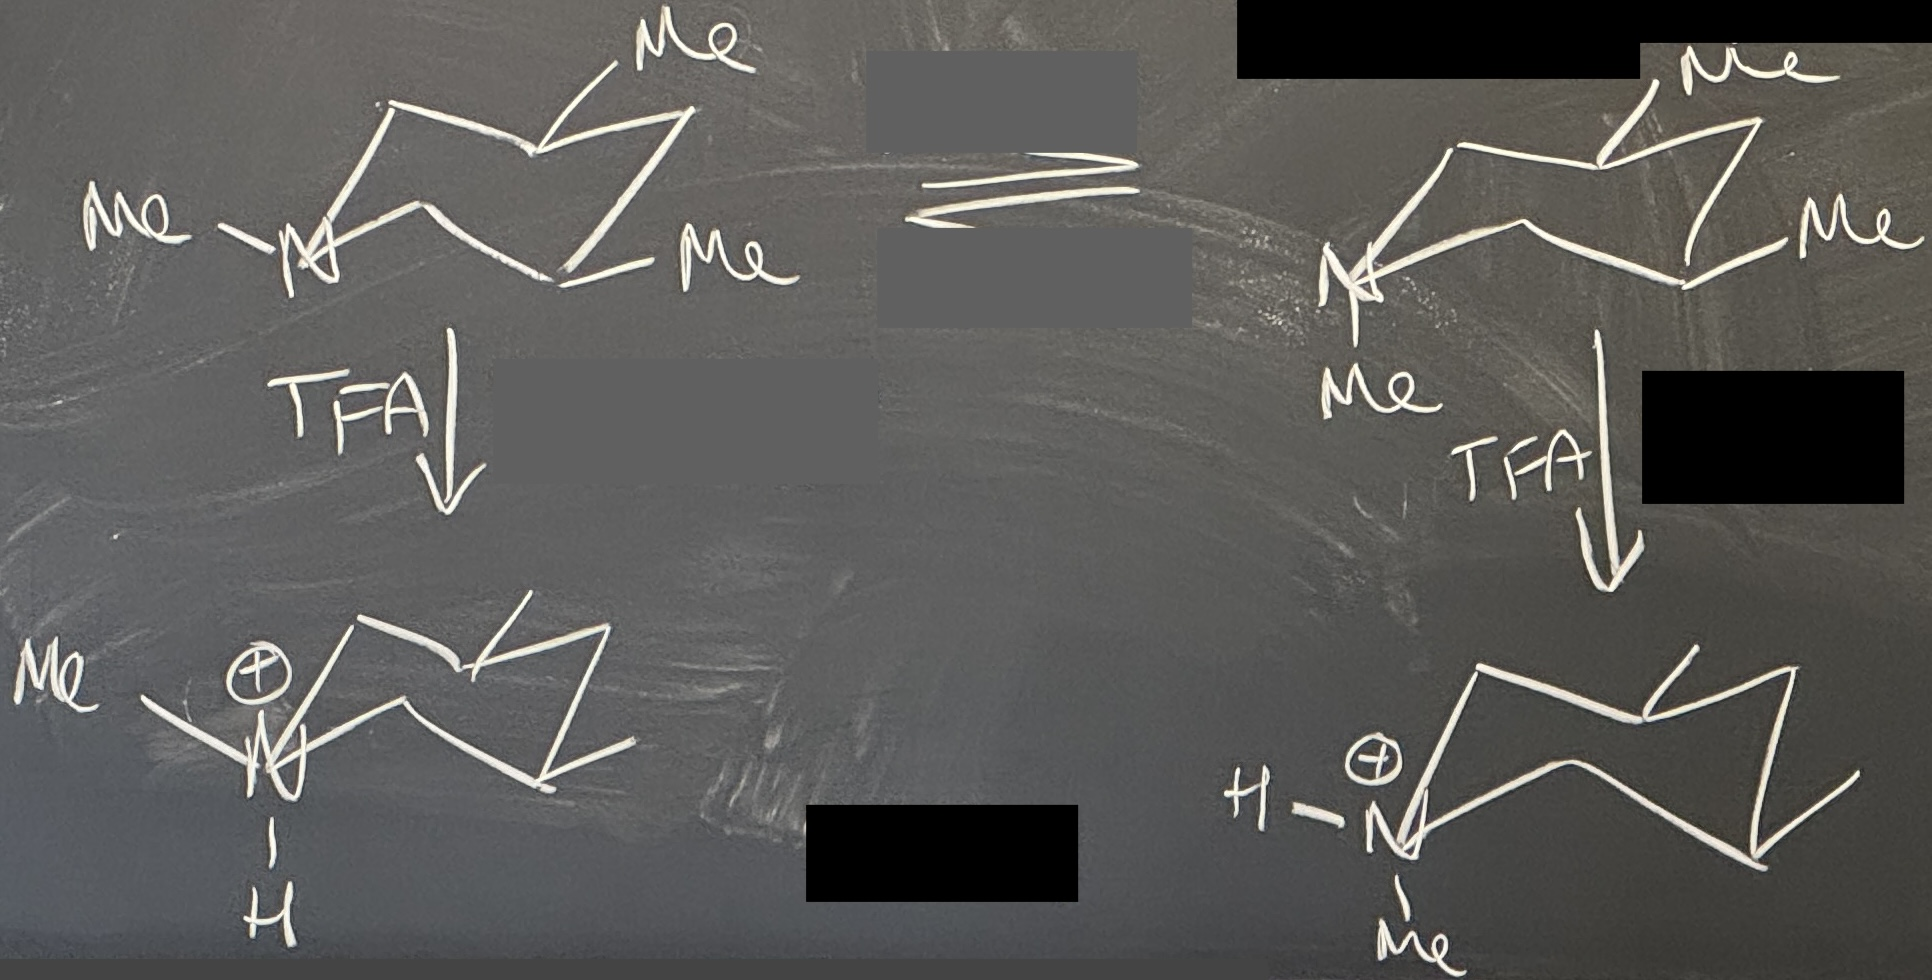
\includegraphics[width=0.45\linewidth]{KQprotonation.JPG}
        \caption{Kinetic quench: Protonation.}
        \label{fig:KQprotonation}
    \end{figure}
    \begin{itemize}
        \item The epimer with the equatorial methyl occurs in a $>15:1$ ratio.
        \item Epimerization occurs relatively slowly, protonation of the equatorial lone pair occurs fast, and protonation of the axial lone pair is even \emph{faster} than protonation of the equatorial one.
        \begin{itemize}
            \item What is "fast" and "slow" is all relative! Usually, nitrogen inversion is fast, but proton transfer (PT) to nitrogen is even faster.
        \end{itemize}
        \item However, the product ratio is also $>15:1$, just like the SM ratio. To reiterate, this is because we're not interconverting between our starting materials.
    \end{itemize}
    \item Moving on, let's discuss the \textbf{principle of microscopic reversibility}.
    \item \textbf{Principle of microscopic reversibility}: The lowest energy path connecting two intermediates is the same, regardless of the direction in which the reaction proceeds.
    \begin{itemize}
        \item Basically, if you propose a mechanism from \ce{A -> B}, the same mechanism (in reverse) has to be true for \ce{B -> A}.
        \item If we proceed through a certain transition state in one direction, we cannot proceed through a different transition state on the way back.
        \item Really useful to probe kinetically silent steps.
    \end{itemize}
    \item A cool example of using the principle of microscopic reversibility to see which mechanism is operative (Figure \ref{fig:MicroReverMech}).
    \begin{figure}[h!]
        \centering
        \begin{subfigure}[b]{\linewidth}
            \centering
            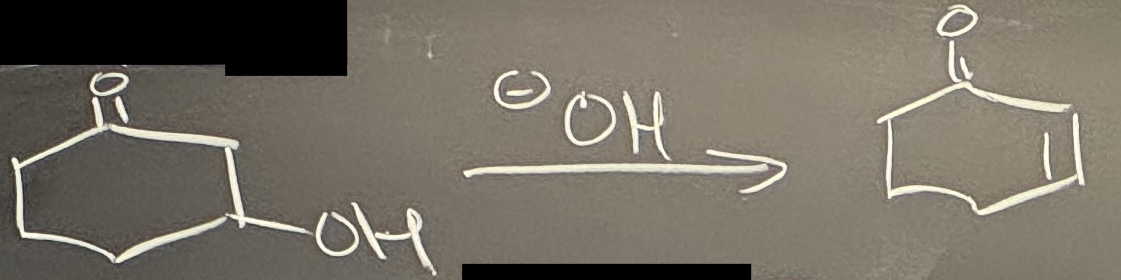
\includegraphics[width=0.25\linewidth]{MicroReverMecha.JPG}
            \caption{An elimination reaction.}
            \label{fig:MicroReverMecha}
        \end{subfigure}\\[2em]
        \begin{subfigure}[b]{0.49\linewidth}
            \centering
            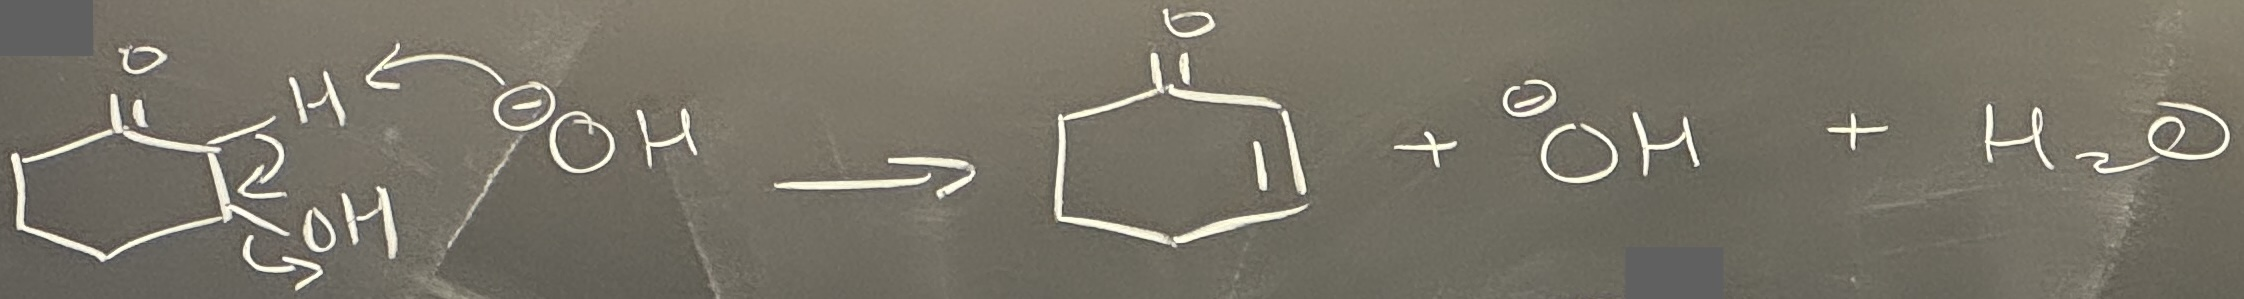
\includegraphics[width=0.95\linewidth]{MicroReverMechb.JPG}
            \caption{E\textsubscript{2} mechanism.}
            \label{fig:MicroReverMechb}
        \end{subfigure}
        \begin{subfigure}[b]{0.49\linewidth}
            \centering
            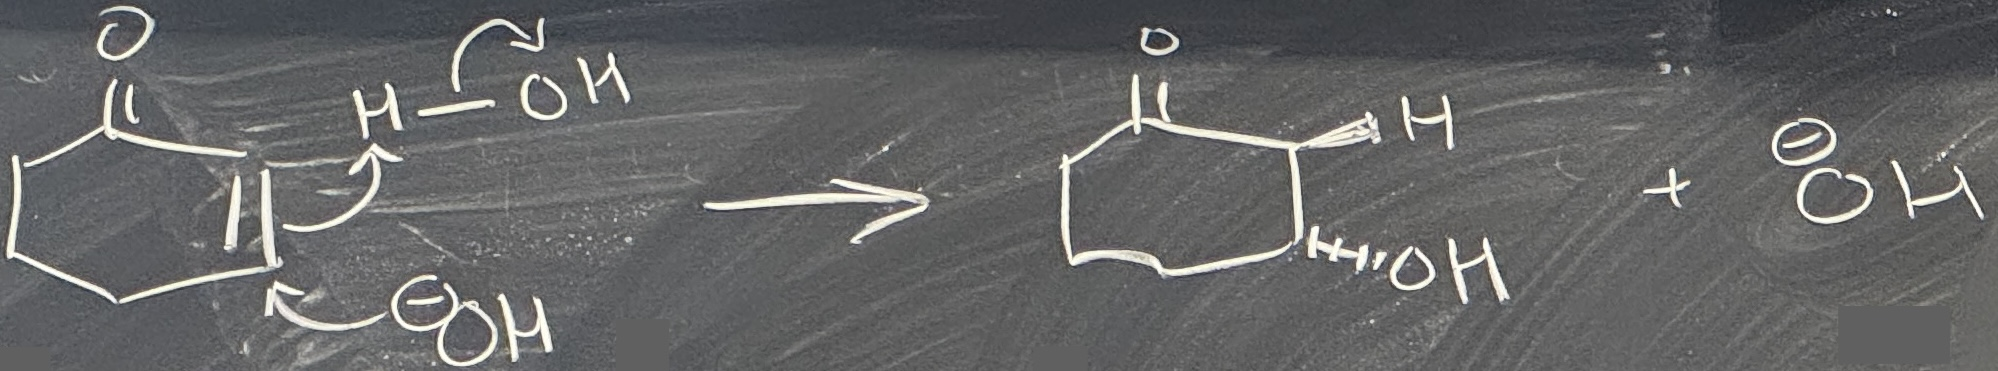
\includegraphics[width=0.82\linewidth]{MicroReverMechc.JPG}
            \caption{Retro-E\textsubscript{2} mechanism.}
            \label{fig:MicroReverMechc}
        \end{subfigure}\\[2em]
        \begin{subfigure}[b]{0.49\linewidth}
            \centering
            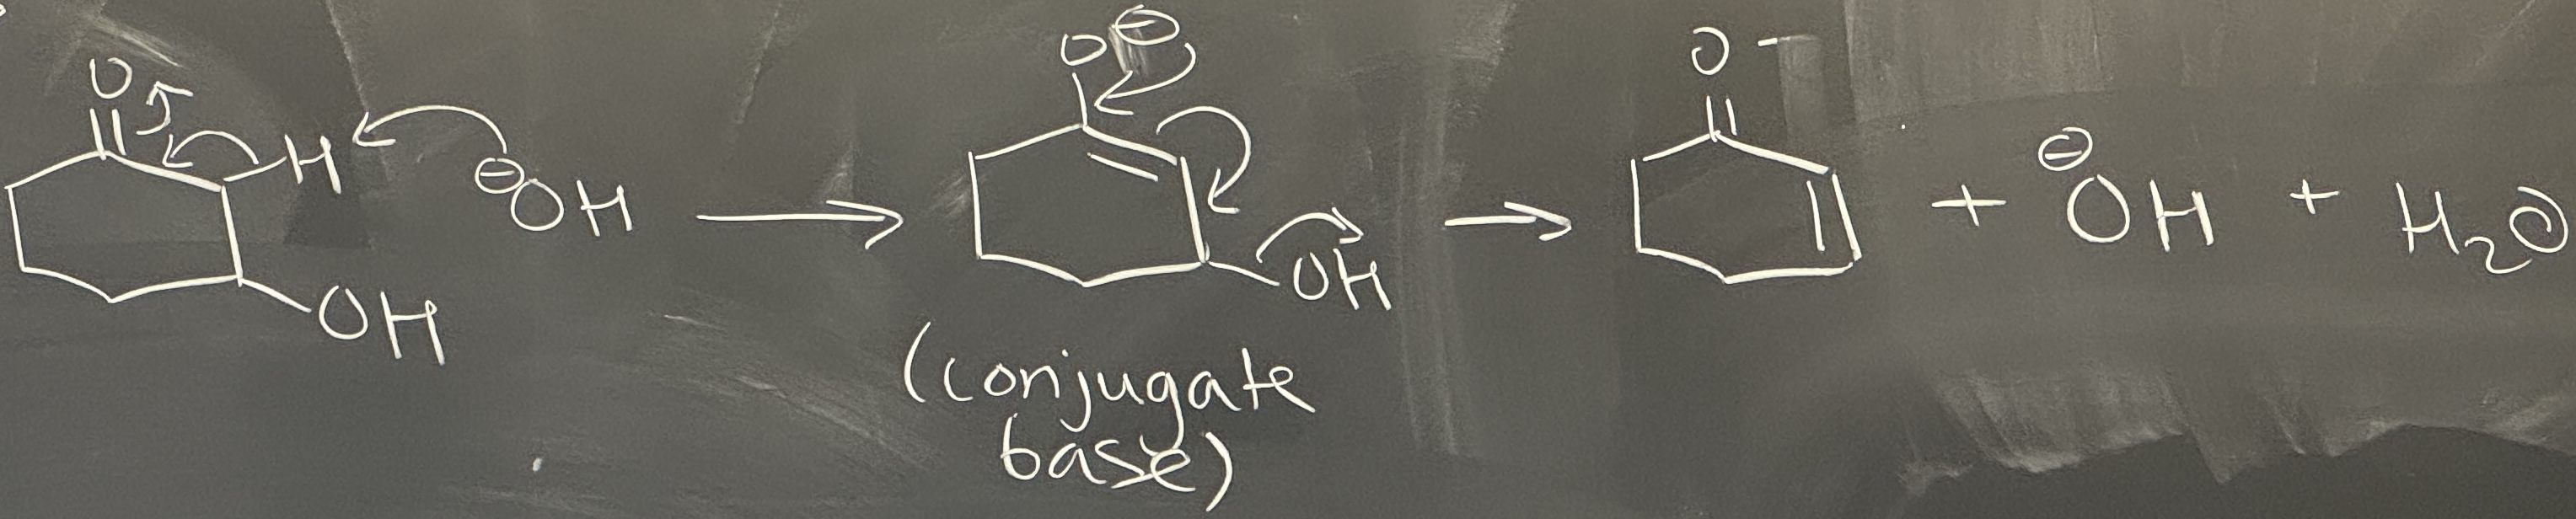
\includegraphics[width=\linewidth]{MicroReverMechd.JPG}
            \caption{E\textsubscript{1}CB mechanism.}
            \label{fig:MicroReverMechd}
        \end{subfigure}
        \begin{subfigure}[b]{0.49\linewidth}
            \centering
            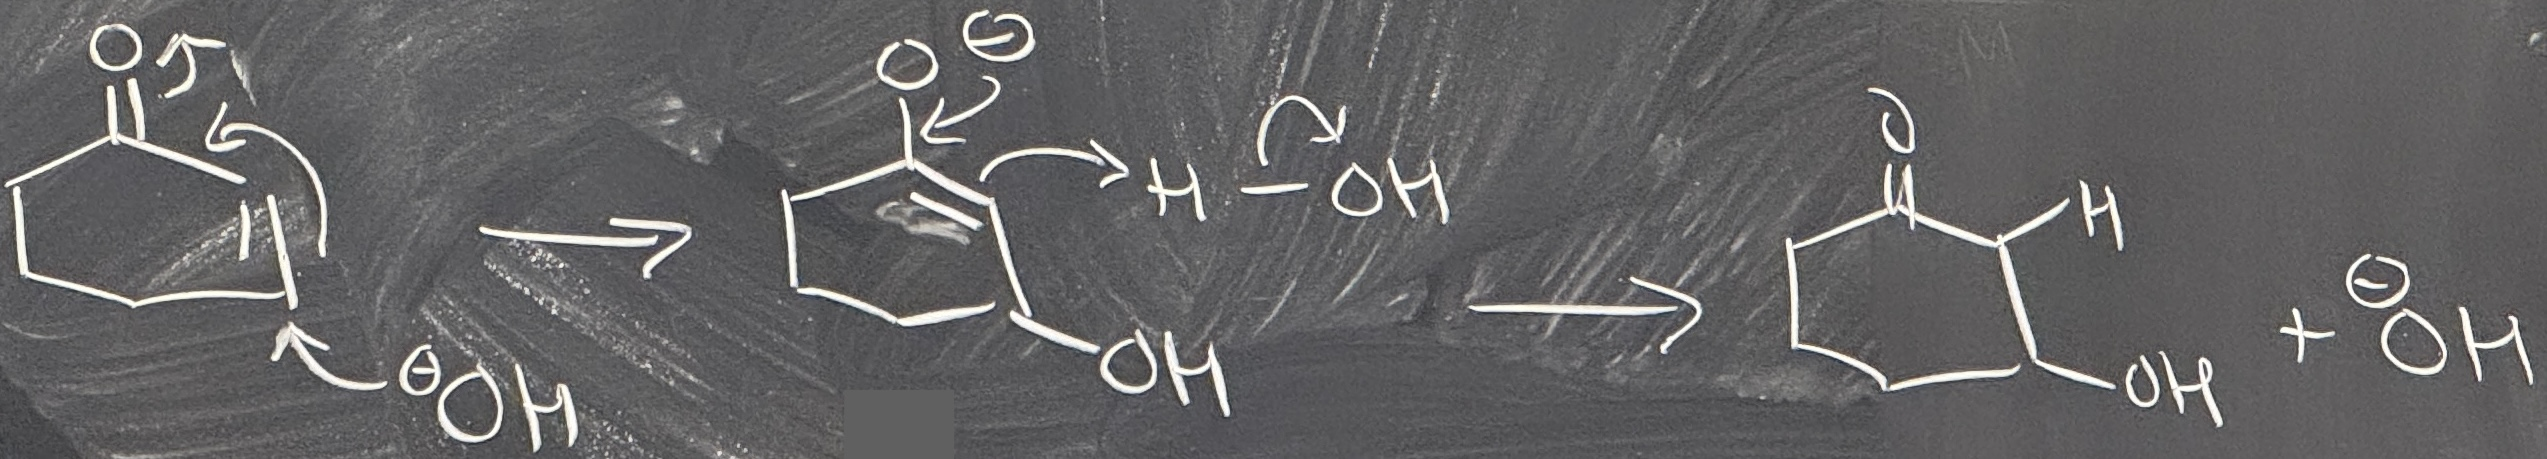
\includegraphics[width=0.95\linewidth]{MicroReverMeche.JPG}
            \caption{Retro-E\textsubscript{1}CB mechanism.}
            \label{fig:MicroReverMeche}
        \end{subfigure}
        \caption{Microscopic reversibility to differentiate plausible mechanisms.}
        \label{fig:MicroReverMech}
    \end{figure}
    \begin{itemize}
        \item Consider the elimination of a $\beta$-hydroxyketone to form an enone (Figure \ref{fig:MicroReverMecha}).
        \item Is the mechanism E\textsubscript{2} (Figure \ref{fig:MicroReverMechb}) or \textbf{E\textsubscript{1}CB} (Figure \ref{fig:MicroReverMechd})?
        \item How can we determine the better mechanism? Consider the reverse reactions!
        \begin{itemize}
            \item Retro-E\textsubscript{2} (Figure \ref{fig:MicroReverMechc}): A one-step forward reaction for E\textsubscript{2} means a one-step reverse reaction, wherein \ce{HO-} adds in, the olefin grabs a proton from water, and \ce{HO-} leaves.
            \item Retro-E\textsubscript{1}CB (Figure \ref{fig:MicroReverMeche}): This time, a two-step reverse reaction is implied. First, we kick electron density all the way up to oxygen, and second, we kick arrows back down to grab a proton.
        \end{itemize}
        \item Which reverse mechanism is more plausible?
        \begin{itemize}
            \item In Figure \ref{fig:MicroReverMechc}, we need a termolecular transition state (which is possible, but rare). However, we'd also form only the anti product, and this is flatly inconsistent with experiment.
            \item In Figure \ref{fig:MicroReverMeche}, we have a conjugate addition step followed by an enolate protonation step, both of which are very typical reactions.
            \begin{itemize}
                \item Molecular orbital theory also implies that the electrons push all the way up through the conjugated system to the oxygen in a concerted step upon nucleophilic addition at the B\"{u}rgi-Dunitz angle, like in 5.13!
            \end{itemize}
        \end{itemize}
        \item Now remember that the more reasonable mechanism must follow the same steps in the forward and reverse direction.
        \begin{itemize}
            \item Thus, more reasonable in reverse implies more reasonable in forward!
        \end{itemize}
        \item Conclusion: E\textsubscript{1}CB wins!
    \end{itemize}
    \item \textbf{Elimination unimolecular conjugate base}: Just a type of E1 that happens with an acidic proton. \emph{Also known as} \textbf{E\textsubscript{1}CB}.
    \begin{itemize}
        \item You draw the formation of a conjugate base (i.e., the conjugate base of the SM "acid") followed by the elimination of something.
    \end{itemize}
    \item That wraps it up for microscopic reversibility; let's now move onto another principle.
    \item \textbf{Reactivity-selectivity principle}: It is often observed that a more reactive reactant, intermediate, or reagent corresponds to a less selective reaction.
    \begin{itemize}
        \item When we say "more reactive," we typically mean higher energy, more exothermic, etc.
        \item This happens because the transition states to different products tend to resemble this higher energy intermediate per the \textbf{Hammond postulate}.
        \item It follows since the transition state does not resemble the products that it is less sensitive to differences in product energy, so it is harder for the transition state to differentiate between products, so the reaction is less selective.
    \end{itemize}
    \item \textbf{Hammond postulate}: The transition state is most similar in structure to the higher energy intermediate.
    \item Example of the reactivity-selectivity principle: Radical halogenation.
    \begin{figure}[h!]
        \centering
        \footnotesize
        \schemestart
            \chemfig{-[:30](-[2])-[:-30]-[:30]}
            \arrow(.-10--){->[\ce{X2}][$h\nu$]}
            \chemfig{-[:30](-[:110])(-[:70]X)-[:-30]-[:30]}
            \+{,,0.7em}
            \chemfig{-[:30](-[2])-[:-30](-[6]X)-[:30]}
            \+
            \chemfig{-[:30](-[2]-[:30]X)-[:-30]-[:30]}
            \+
            \chemfig{-[:30](-[2])-[:-30]-[:30]-[:-30]X}
        \schemestop
        \caption{Reactivity-selectivity principle in radical halogenation.}
        \label{fig:reactSelect}
    \end{figure}
    \begin{itemize}
        \item This reaction yields 1 tertiary product, 2 different secondary products, and 1 primary product.
    \end{itemize}
    \item The reaction in Figure \ref{fig:reactSelect} forms diffferent product distributions with different halogens.
    \begin{table}[h!]
        \centering
        \small
        \renewcommand{\arraystretch}{1.2}
        \setchemfig{atom sep=1em,bond offset=1pt,fixed length=false,atom style={font=\tiny},bond style=thick}
        \begin{tabular}{c|cccc}
             & \chemfig{-[:30](-[:110])(-[:70]\textbf{X})-[:-30]-[:30]}
                & \chemfig{-[:30](-[2])-[:-30](-[6]\textbf{X}-[6,0.5,,,opacity=0])-[:30]}
                & \chemfig{-[:30](-[2]-[:30]\textbf{X})-[:-30]-[:30]}
                & \chemfig{-[:30](-[2])-[:-30]-[:30]-[:-30]\textbf{X}}\\
            \hline
            $\bm{\textbf{X}=\textbf{Cl}}$ \textbf{(\%)} & 28 & 35 & 24 & 12\\
            $\bm{\textbf{X}=\textbf{Br}}$ \textbf{(\%)} & 90 & 9 & $<1$ & $<1$\\
        \end{tabular}
        \caption{Product distribution in radical bromination vs. chlorination.}
        \label{tab:reactSelect}
    \end{table}
    \begin{itemize}
        \item Evidently, \ce{Br*} is more selective than \ce{Cl*}.
    \end{itemize}
    \item Why? Consider BDEs in the selectivity-determining propagation step wherein a halide radical creates an alkyl radical and \ce{HCl}.
    \begin{figure}[h!]
        \centering
        \begin{subfigure}[b]{0.35\linewidth}
            \centering
            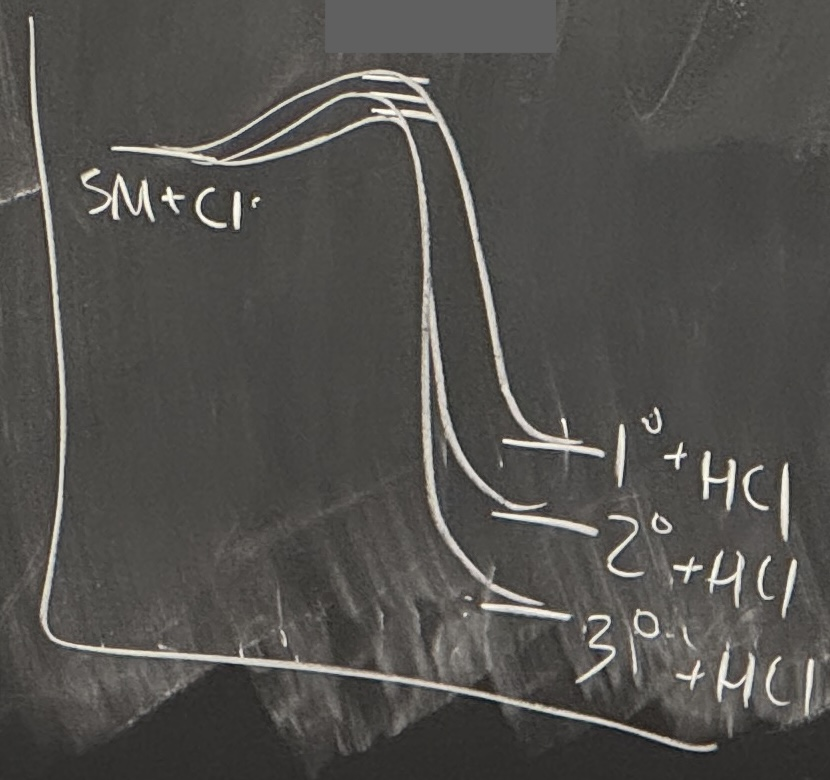
\includegraphics[width=0.7\linewidth]{Hammonda.JPG}
            \caption{Chlorination energy diagram.}
            \label{fig:Hammonda}
        \end{subfigure}
        \begin{subfigure}[b]{0.35\linewidth}
            \centering
            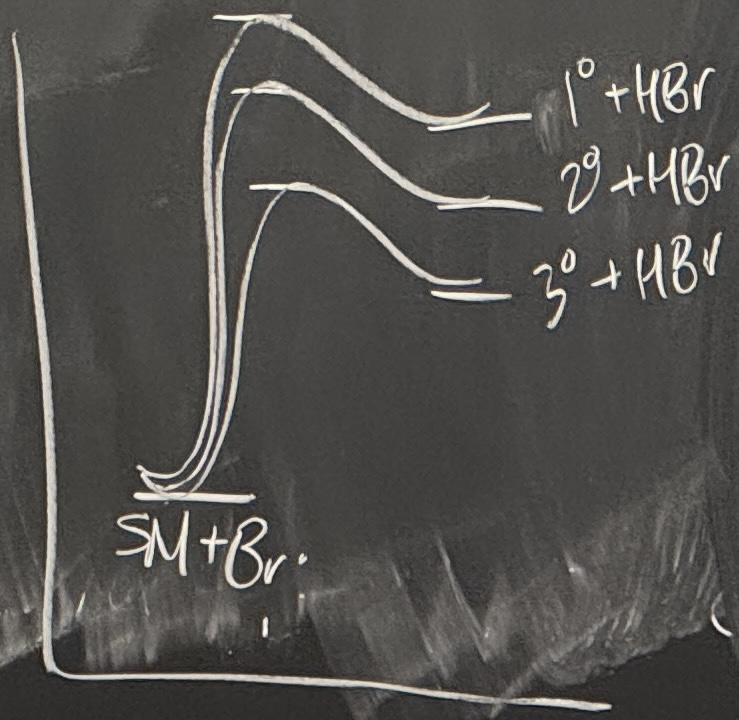
\includegraphics[width=0.68\linewidth]{Hammondb.JPG}
            \caption{Bromination energy diagram.}
            \label{fig:Hammondb}
        \end{subfigure}
        \caption{The Hammond postulate explains the reactivity-selectivity principle.}
        \label{fig:Hammond}
    \end{figure}
    \begin{itemize}
        \item In radical chlorination: \ce{C-H} has a BDE of \kcal{98} and \ce{H-Cl} has a BDE of \kcal{103}.
        \begin{itemize}
            \item Thus, the reaction is exothermic with $\Delta H=-\kcal{5}$.
            \item Then per the reactivity-selectivity principle, we have a high-energy intermediate. This will lead to three energetically close transition states that unselectively determine the product (Figure \ref{fig:Hammonda}).
        \end{itemize}
        \item In radical bromination: \ce{C-H} has a BDE of \kcal{98} and \ce{H-Br} has a BDE of \kcal{87}.
        \begin{itemize}
            \item Thus, the reaction is endothermic with $\Delta H=\kcal{11}$.
            \item Then per the reactivity-selectivity principle, we have a low-energy intermediate. This will lead to three energetically distinct transition states that resemble the product more and hence selectively determine it (Figure \ref{fig:Hammondb}).
        \end{itemize}
        \item The reactivity-selectivity principle is useful to understand and many-times true, but there are also many exceptions.
        \begin{itemize}
            \item Example exception: If there are more complicated mechanistic relationships between the SMs and transition states.
        \end{itemize}
        \item See Figure 3.4 of \textcite{bib:CHEM22100Notes}!
    \end{itemize}
    \item Practical aspects of selectivity (will come up on our quals).
    \begin{itemize}
        \item Numbers worth knowing.
        \item We'll go over this in the Lecture 10 recap on Thursday!
    \end{itemize}
\end{itemize}



\section{Office Hours (Jonathan)}
\begin{itemize}
    \item Would this similarly predict that \ce{H2O} has longer bonds than \ce{NH3}?
    \begin{itemize}
        \item Perhaps, but other factors make \ce{O-H} bonds in water shorter than the \ce{N-H} bonds in ammonia.
    \end{itemize}
    \item In what way does the HIA only tell us the \emph{relative} stability?
    \begin{itemize}
        \item The number doesn't tell us anything on its own, and it's not a very useful number.
        \item Essentially, all we can learn from these is which cations are more reactive \emph{relative} to other cations.
    \end{itemize}
    \item How can \ce{Bn-Br} be the most stable and most reactive species (Table \ref{tab:HIAk})?
    \begin{itemize}
        \item The benzyl \emph{cation} (not the benzyl bromide) is the most stable because it takes the least energy to create it. We had to put more energy into the other two systems to create carbocations, so they are higher energy and hence less stable.
        \item The benzyl cation is most reactive toward solvolysis because it has the highest $\krel$.
    \end{itemize}
    \item Mayr electrophilicity?
    \begin{itemize}
        \item What I wrote down sounds wrong to Jonathan.
        \item It has nothing to do with the thermodynamic stability of anything; it's all about rate constants.
        \item I can read the paper if I want, but it's probably not too important.
    \end{itemize}
\end{itemize}




\end{document}